Looking beyond simple token delivery, companies can start building solutions that operate without implicit trust, fully aligning with Zero Trust principles. 
This approach is particularly well-suited for Zero Trust Network Access (ZTNA) and the emerging requirements of AI agents.  

In this scope, there are significant business opportunities.  
Enterprises will need new forms of \textbf{Zero Trust governance}, capable of auditing and controlling authorization decisions in real time.  
A new generation of \textbf{Policy Decision Points (PDPs)} can enable innovative products around trust evaluation and enterprise decision governance.  

In parallel, logging providers will play a central role by developing tools to capture, analyze, and interpret decision logs.  
As highlighted by Wardley Maps, while \textbf{policy languages} are rapidly becoming commoditized, the true differentiators will be stronger \textbf{trust models}, \textbf{dynamic permissions}, and advanced \textbf{anomaly detection}.  

\begin{figure*}[htbp]
    \centering
    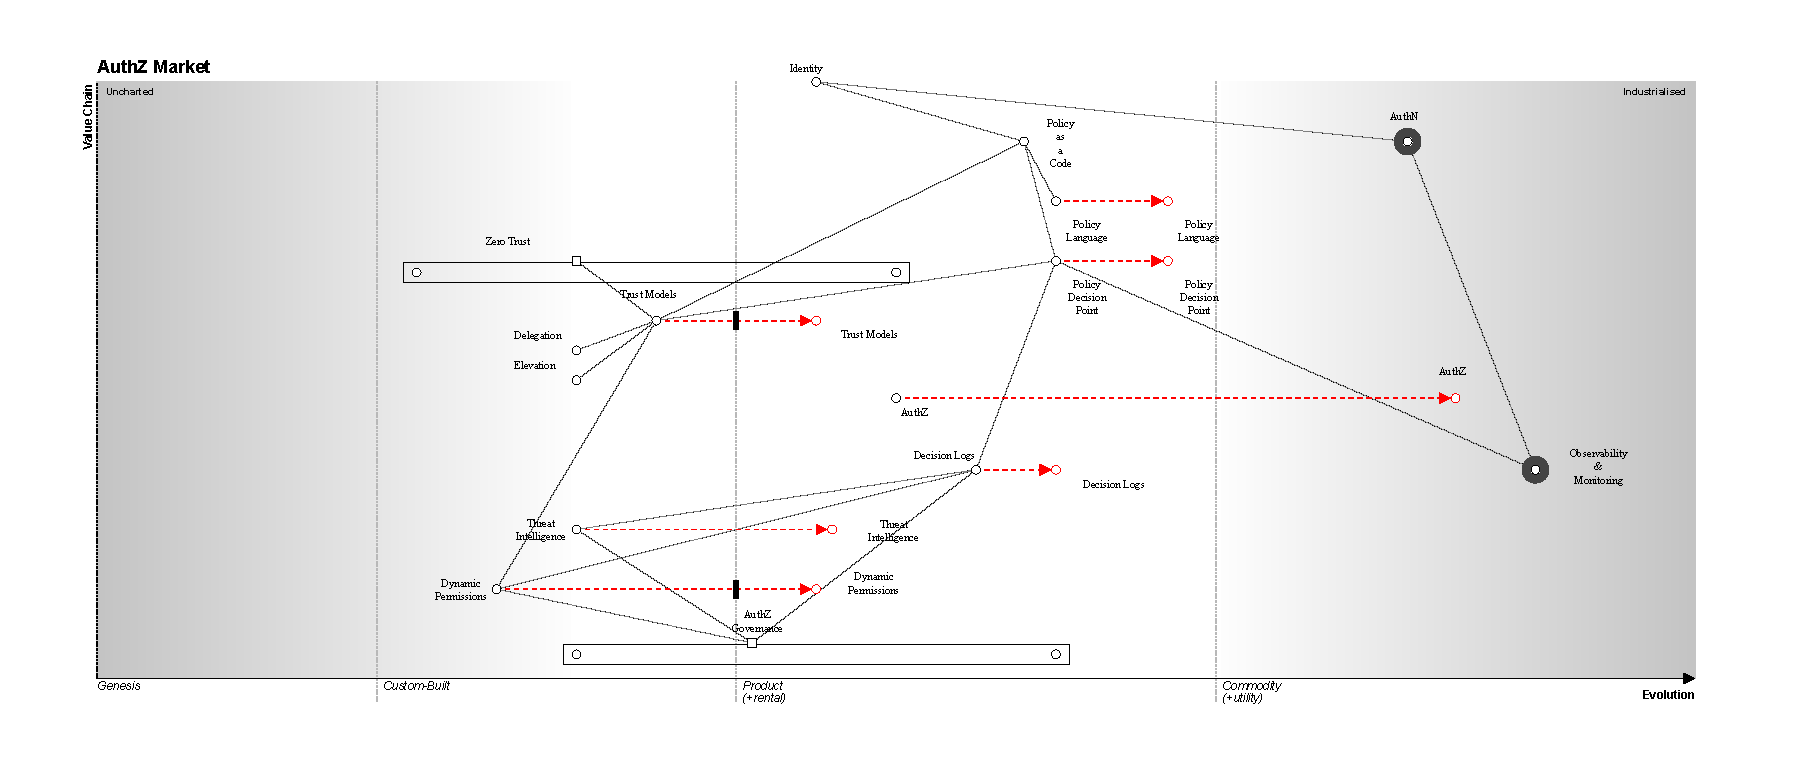
\includegraphics[width=0.9\textwidth]{market/wardley-maps.pdf}
    \caption{Wardley Maps for Zero Trust AuthZ}
    \label{fig:wardley-maps-enterprise}
\end{figure*}

This ecosystem will be essential to manage AI agents.  
Agents will connect to existing applications and extend them with intelligent capabilities, but companies will still need a unified solution to govern their software landscape.  
For this reason, a next-generation Zero Trust authorization protocol is required to achieve the next level of security and governance.

